\documentclass[11pt,a4paper,openright,twoside]{extreport}
\usepackage[utf8]{inputenc}
\usepackage[english]{babel}
\usepackage[inner=2cm,outer=2cm,top=2cm,bottom=2cm]{geometry}
\usepackage{amsmath}
\usepackage{amsfonts}
\usepackage{textcomp}
\usepackage{amssymb}
\usepackage{pifont}
\usepackage{epstopdf}
\usepackage[singlespacing]{setspace}
\usepackage{tabularx}
\usepackage{mathrsfs}
\usepackage{rotating}
\usepackage{caption}
\usepackage[usenames,dvipsnames]{xcolor}
\usepackage{fancyref}
\usepackage{subcaption}
\usepackage{braket}
\usepackage{color}
\usepackage{float}
\usepackage{enumerate}
\usepackage[pagebackref]{hyperref}
\usepackage{afterpage}
\usepackage[makeroom]{cancel}

\usepackage{fancyhdr}
\pagestyle{fancy}

\usepackage{graphicx}
\usepackage{subcaption}
\usepackage{wrapfig}
\graphicspath{{images/}}

\fancyhead{}
\fancyhead[RE, LO]{{\nouppercase{\rightmark{Dhole, Mensing, Padalkar}}}}
\fancyhead[LE, RO]{\thepage}
\setlength{\headheight}{15pt}
\renewcommand{\headrulewidth}{0.4pt}

\fancyfoot{}
\fancyfoot[RE, LO]{{\nouppercase{\leftmark{MAS-SS18 | Hochschule Bonn-Rhein-Sieg}}}}
\fancyfoot[LE, RO]{Date: 26.04.2017}
\renewcommand{\footrulewidth}{0.4pt}

\hypersetup{
    pdftoolbar=true,        % show Acrobat’s toolbar?
    pdfmenubar=true,        % show Acrobat’s menu?
    pdffitwindow=false,     % window fit to page when opened
    pdfstartview={FitH},    % fits the width of the page to the window
    pdftitle={Scientific Experimentation and Evaluation Homework},    % title
    pdfauthor={Pranjal Dhole},     % author
    pdfsubject={Review},   % subject of the document
    pdfcreator={Pranjal Dhole},   % creator of the document
    pdfproducer={Pranjal Dhole}, % producer of the document
    pdfkeywords={SEEHomework} {Scientific Experimentation and Evaluation}, % list of keywords
    pdfnewwindow=true,      % links in new window
    colorlinks=true,       % false: boxed links; true: colored links
    linkcolor=MidnightBlue, % color of internal links (change box color with linkbordercolor)
    citecolor=Thistle,        % color of links to bibliography
    filecolor=magenta,      % color of file links
    urlcolor=Sepia           % color of external links
}
%%%%%%%%%%%%%%%%%%%%%%%%%%%%%%%%%%%%%%%%%%%%%%%%%%%%%%%%%%%%%%%%%%%%%%%%%%%
%specific
\raggedbottom
%%%%%%%%%%%%%%%%%%%%%%%%%%%%%%%%%%%%%%%%%%%%%%%%%%%%%%%%%%%%%%%%%%%%%%%%%%%
\pagenumbering{arabic}
\begin{document}
%%%%%%%%%%%%%%%%%%%%%%%%%%%%%%%%%%%%%%%%%%%%%%%%%%%%%%%%%%%%%%%%%%%%%%%%%%%
\begin{center}
\section*{\underline{Scientific Experimentation and Evaluation}}

\large{\textbf{Assignment 1.2}}\\
\large{Abhishek Padalkar, Max Mensing, Pranjal Dhole}\\
\large{Due date: Thursday, 26$^{\text{th}}$ April, 2018}
\end{center}

\subsection*{1. Robot configuration}
\label{robot-config}

\begin{figure}[ht]
  \begin{minipage}[b]{0.5\textwidth}
    \centering
    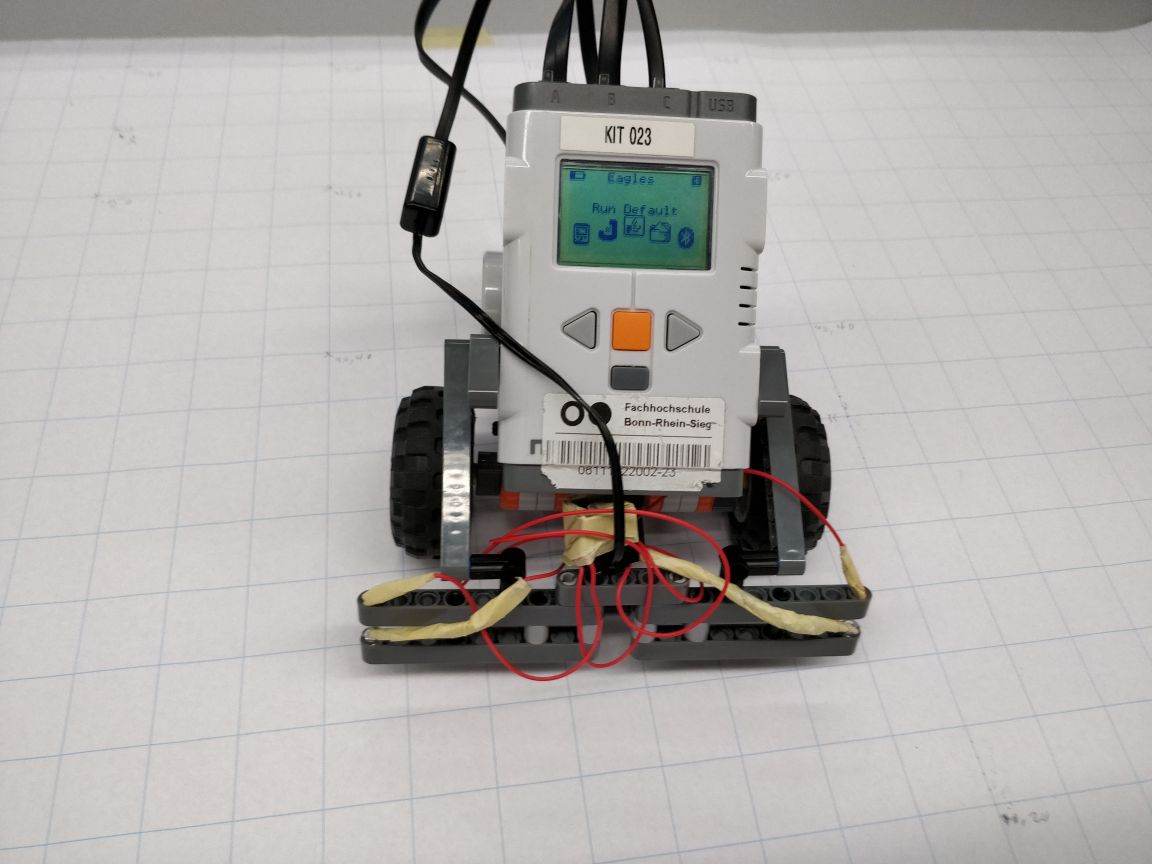
\includegraphics[width=.9\textwidth]{front.jpeg}
    \captionsetup{labelformat=empty}
    \caption{Front view} 
    \vspace{4ex}
  \end{minipage}%%
  \begin{minipage}[b]{0.5\textwidth}
    \centering
    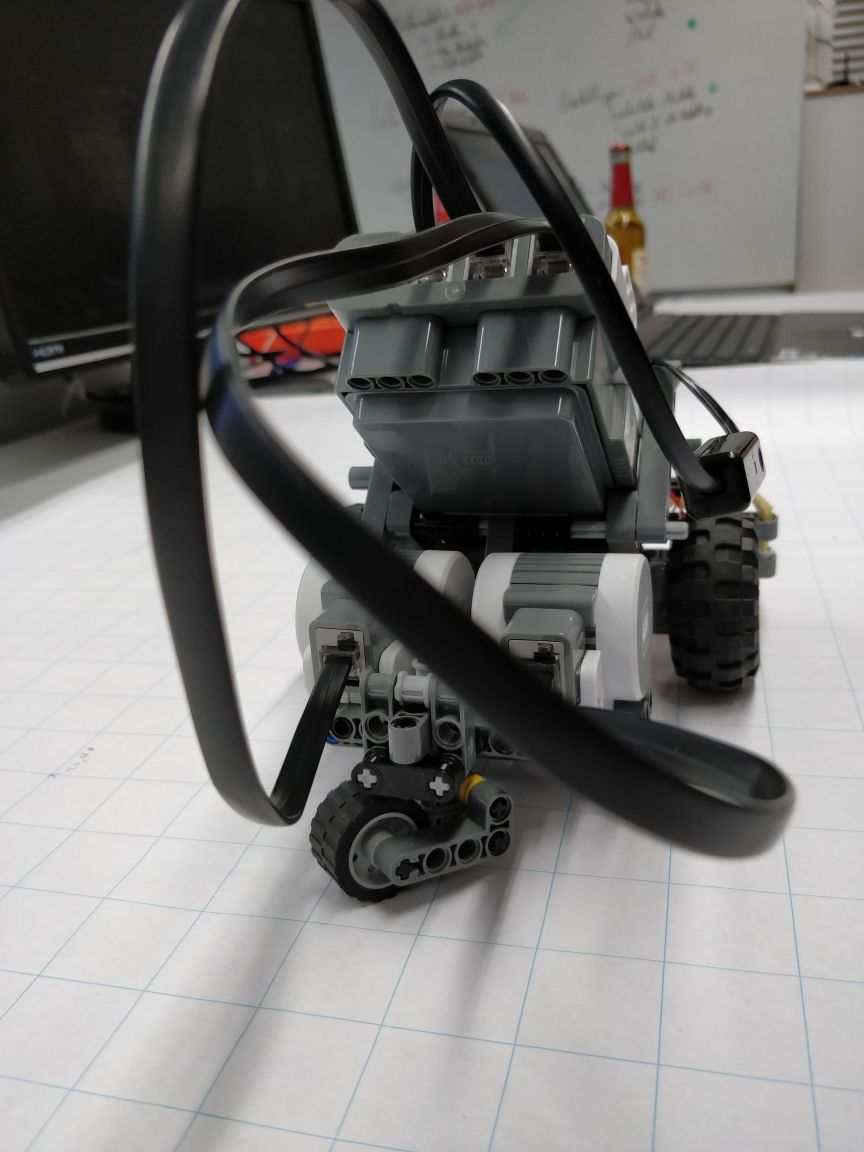
\includegraphics[width=.6\textwidth]{back.jpeg}
    \captionsetup{labelformat=empty}
    \caption{Back view} 
    \vspace{4ex}
  \end{minipage} 
  \begin{minipage}[b]{0.5\textwidth}
    \centering
    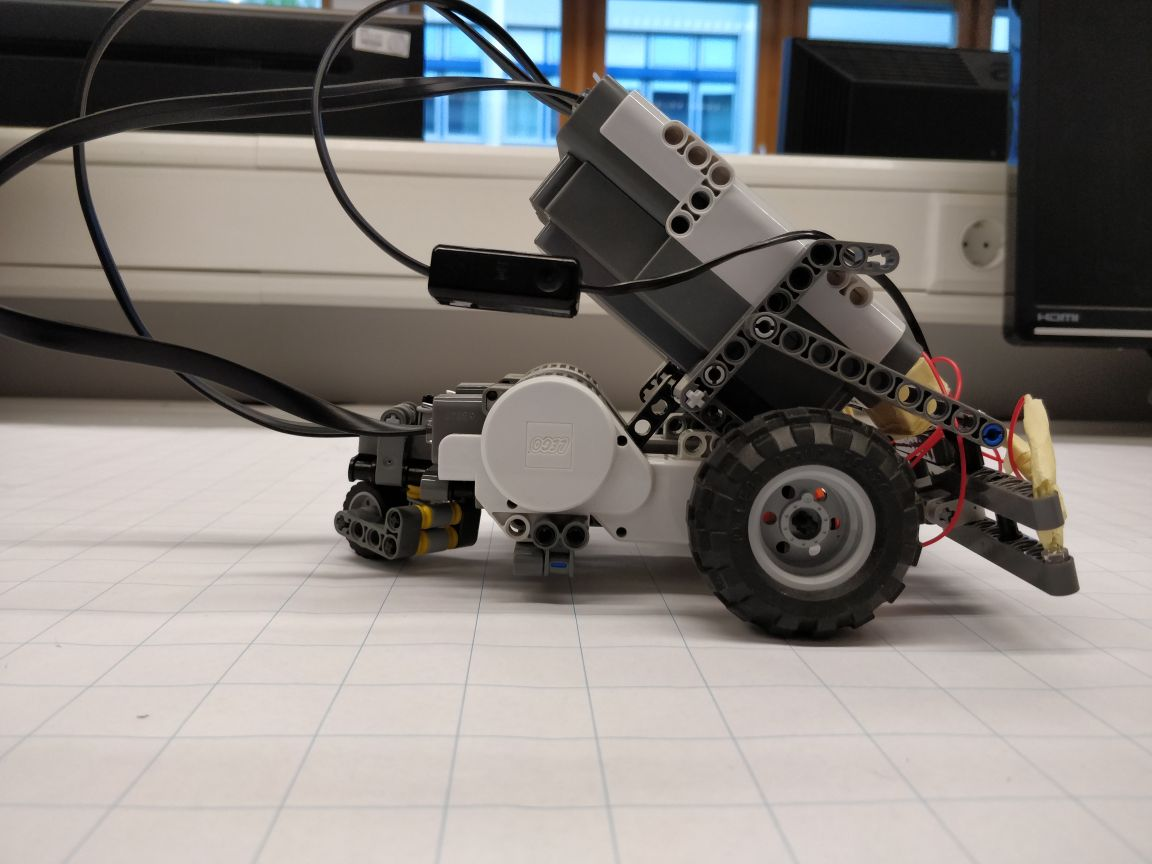
\includegraphics[width=.9\textwidth]{rightSide.jpeg}
    \captionsetup{labelformat=empty}
    \caption{Right side view} 
    \vspace{4ex}
  \end{minipage}%% 
  \begin{minipage}[b]{0.5\textwidth}
    \centering
    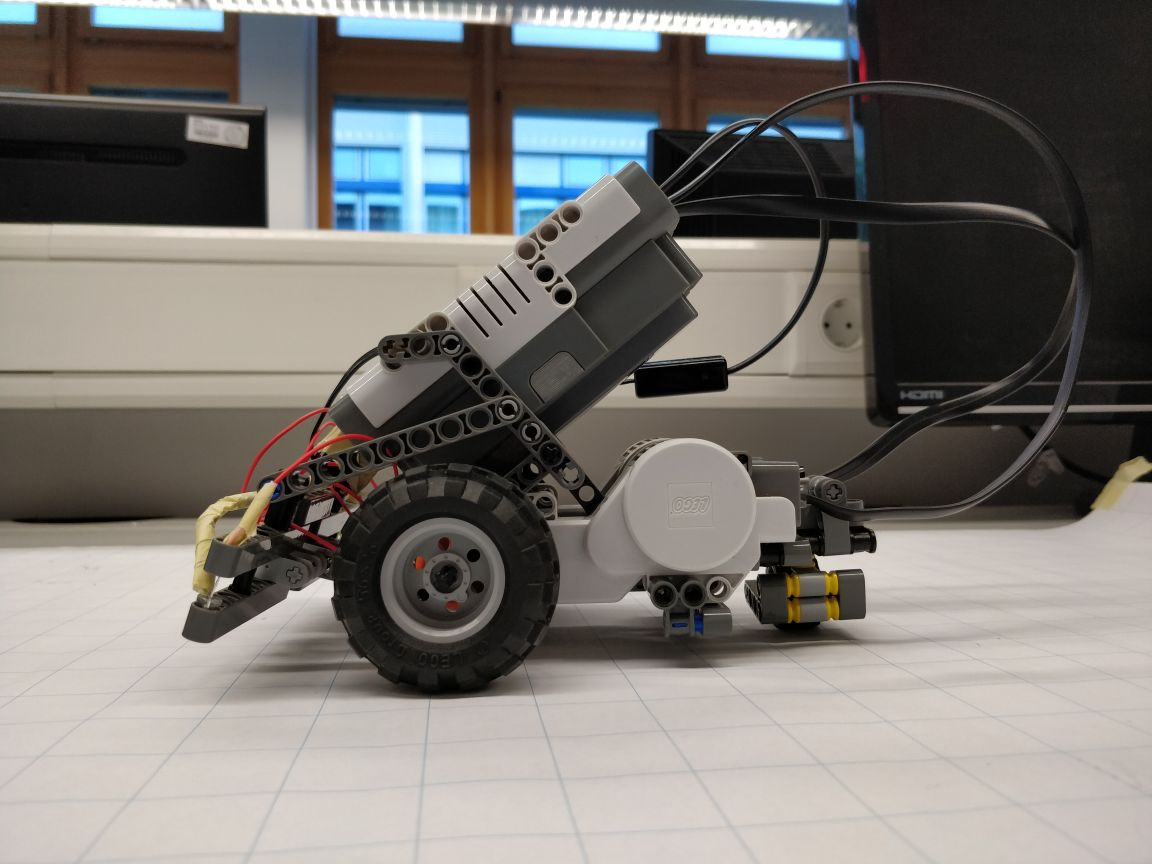
\includegraphics[width=.9\textwidth]{leftSide.jpeg}
    \captionsetup{labelformat=empty}
    \caption{Left side view} 
    \vspace{4ex}
  \end{minipage}
\captionsetup{labelformat=empty}
\caption{Lego robot design}
\end{figure}

\newpage
\subsection*{2. Deliverables 1.2}
\subsubsection*{2.1 Robot design}
\textbf{Materials}
\begin{wrapfigure}{r}{0.4\textwidth}
  \vspace{-50pt}
  \begin{center}
    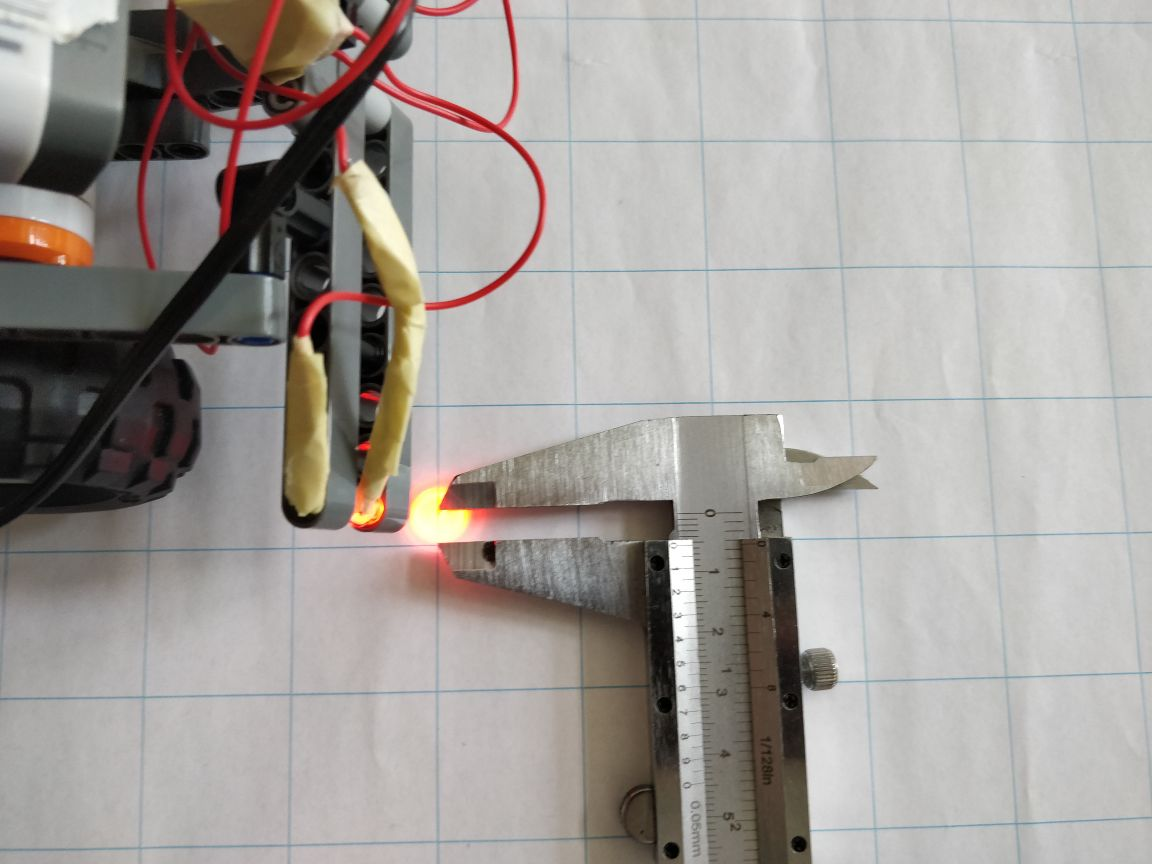
\includegraphics[width=0.39\textwidth]{fringe.jpeg}
  \end{center}
  \vspace{-20pt}
  \caption{Fringes formed on paper by LED lights.}
\end{wrapfigure}

We used the provided Lego Mindstorms 9797 toolkit for the construction of our robot.\\
The robot design is shown in the previous section.\\
For measurement purposes, we have mounted two LED lights with an approx. distance of $9.5 \pm 0.2$ cm in front of the Lego bot. \\
We have attached two resistors of 330 Ohms to each of the LEDs in order to reduce the current flowing through the LEDs. \\
The uncertainty is due to imprecise ruler measurements on each LED. The LED lights formed nice fringes on paper which made marking the center quite easy.\\
We use the provided  2.5x2.5cm grid paper for marking the positions of robot before and after each motion.\\
The corners of the grid paper were glued to the table in order to prevent an movement due to robot motion. 
\subsubsection*{2.2 Experiment}
\begin{itemize}
\item We run the LEGO NXT differential drive robot in three different configurations, viz., straight line motion, right turn motion and left turn motion.
\item The starting position of LEDs is marked on the grid paper and for each trial we align the centres of LED lights on the initial marked position on grid paper.
\item We collected 20 trial data of end robot positions for each configuration.
\item The observations made are tabulated in \texttt{motionData.csv} file attached.
\item The initial position for each configuration run is tabulated in \texttt{motionData\_init.csv} file.
\item In some of the trials the motion initiated in jerks which resulted in larger deviation. These points can be seen as extreme points from the mean of the distribution in each wheel data.
\item Another source of error is the orientation of the back wheel in the initial position. Since it is a passive castor wheel, this could have introduced some discrepancy in the motion.

\begin{figure}[H]
\centering
\begin{subfigure}[b]{0.45\textwidth}
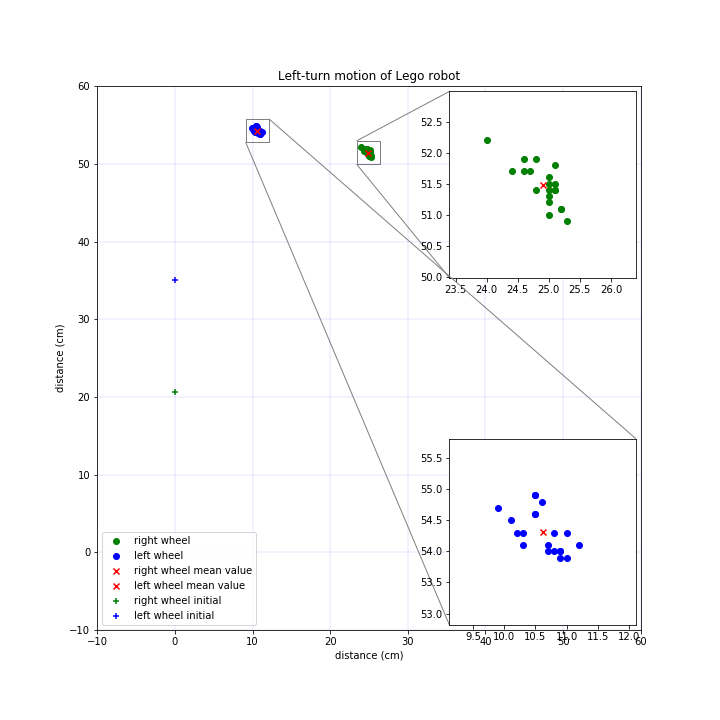
\includegraphics[width=\textwidth]{Left-turn.png}
\caption{Left turn motion}
\label{left}
\end{subfigure}
\begin{subfigure}[b]{0.45\textwidth}
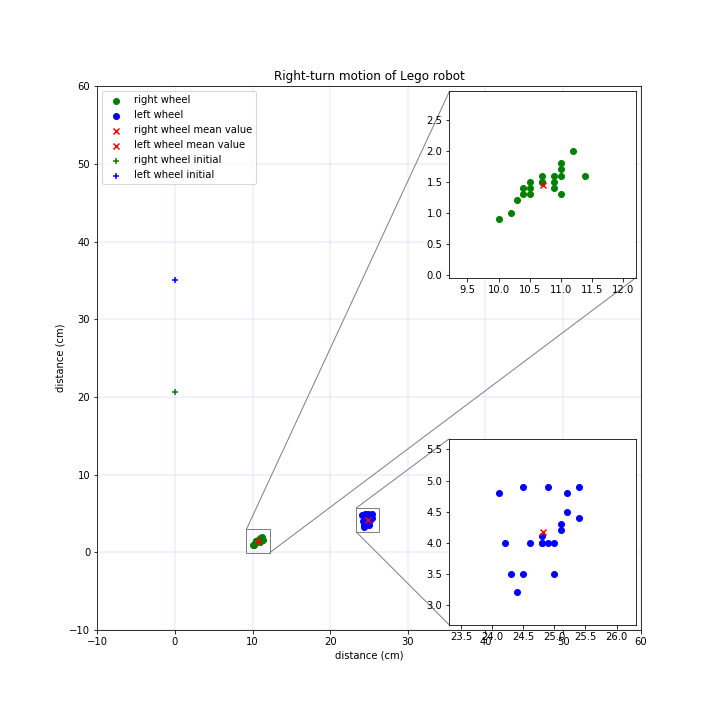
\includegraphics[width=\textwidth]{Right-turn.png}
\caption{Right turn motion}
\label{right}
\end{subfigure}
\begin{subfigure}[b]{0.45\textwidth}
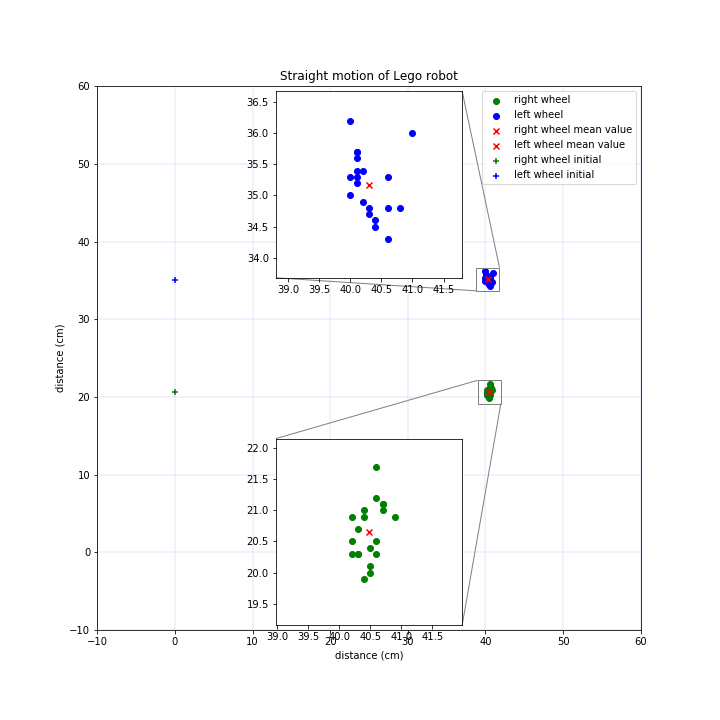
\includegraphics[width=\textwidth]{Straight.png}
\caption{Straight line motion}
\label{straight}
\end{subfigure}
\caption{Robot motion data}
\label{data}
\end{figure}

\item In fig. \ref{data}, the robot motion data is visualized. The initial positions are marked by `+' sign and the mean positions are marked by `x' sign.
\item In fig. \ref{left}, the standard deviation in readings of final wheel position for right and left wheels are (0.3, 0.3) cm and (0.3, 0.3) cm respectively.
\item In fig. \ref{right}, the standard deviation in readings of final wheel position for right and left wheels are (0.3, 0.2) cm and (0.4, 0.5) cm respectively.
\item In fig. \ref{straight}, the standard deviation in readings of final wheel positions for right and left wheels are (0.2, 0.5) cm and (0.3, 0.5) cm respectively.
\item This standard deviation is expected, since there is about 0.2 cm uncertainty in marking the end position of the robot as well as the initial jerky motion introduces some noise.
\item The standard deviations for left and right turn motions are very similar.
\item For straight line motion, we observe a substantial variation in y-readings.
\end{itemize}
%%%%%%%%%%%%%%%%%%%%%%%%%%%%%%%%%%%%%%%%%%%%%%%%%%%%%%%%%%%%%%%%%%%%%%%%%%%%%
\end{document}